\chapter{Proposed implementation}
\label{chap:impl}

My goal is to design and implement library for \acrlong{acc:ea}, as mentioned in the chapter \ref{chap:eva}. The library should not only implement existing \acrshortpl{acc:ea} and allow to execute them on the \gpuns, but also afford general framework to which it would be simple to plug new algorithms. For the user of the library should be easy to replace evolutionary operators, modify them or if necessary replace the whole workflow of the algorithm.

I decide to implement the library using Pipe and Filter architecture as specified by \citet{EnterpriseIntegrationPatterns}. The example of this architecture is in figure \ref{fig:pipesandfilters}. The general idea is to partition the algorithm into smaller, simple steps and use the output of one step as the input to the following one. \acrshort{acc:ea} are simple to split, as one step may be one evolutionary operator. I decided to implement the library in the \enquote{Convention over Configuration} design pattern -- that is the operators make same assumptions about the format and order of the input, rather than explicitly specifying it in the configuration. I still provide ways to control the parameters, if required by the user, and I will get to it a bit later.

\begin{figure}
    \centering
    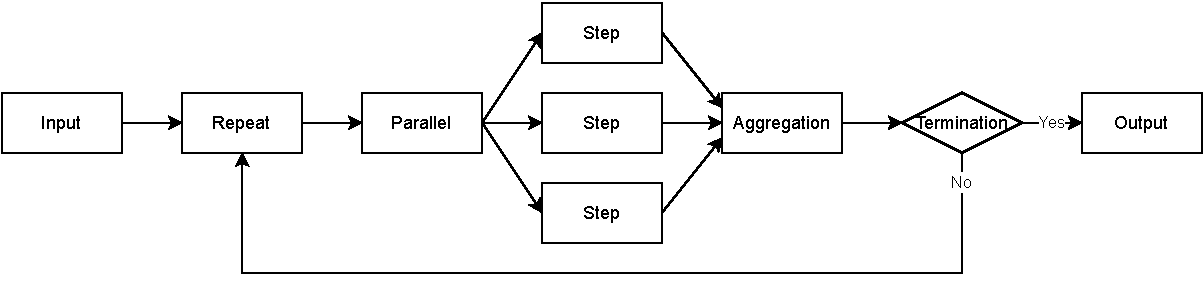
\includegraphics[width=\textwidth]{img/PipesAndFilters.pdf}
    \caption{Pipe and Filter architecture}
    \label{fig:pipesandfilters}
\end{figure}

The pure Pipe and Filter architecture is not sufficient for implementation of \acrshort{acc:ea}. In the purest implementation, this architecture is just chain of steps following each other. I decide to expand it by a number of useful steps like loops, parallel step invocation and more. Example of parallel step respectively loop use in the Pipe and Filter architecture is demonstrated in figure \ref{fig:pipesandfilters}. The parallel invocation is designed in the figure by \enquote{Parallel} block, followed by the \enquote{Aggregation} block accumulating the results from each step. The loop is represented by the \enquote{Repeat} block accompanied by the \enquote{Termination} block controlling the termination condition of the loop.

My proposed implementation is the \emph{\acrfull{acc:ffeat}}. This library is attached to this work, available on my GitHub account \citep{FFEATrepo}, and ready for install as PyPI (Python Package Index) \href{https://pypi.org/project/FFEAT/}{package}. The PyPI is de facto standard way of installing Python packages from a central repository.

As I mentioned earlier, I decided to implement the library in the PyTorch library and Python programming language. Python allows invocation of function with variable number of arguments and variable number of keyword arguments. Without explaining it into too much detail, arguments are passed into the function as in a list and depends on their order. These are the traditional arguments known from languages like C and \cppns. Keyword arguments must be specified by their parameter name. The following line of code invokes function \textit{some\_function} with two parameters $1$ and $2$, and a keyword argument $karg=5$.

\begin{lstlisting}[language=Python]
some_function(1, 2, karg=5)
\end{lstlisting}

I use this design to implement operators in Pipe and Filter architecture. Operator accepts variable number of normal and keyword arguments, and returns list of variables and a dictionary. The list of variables, respectively the dictionary serves as the input for the following operator as normal, respectively as keyword arguments. Following this design, new operator may be easily plug in into the algorithm. At the same time, it allows to use the same underlying architecture both for genetic algorithms (the argument is only the population), as well as \acrshort{acc:pso} algorithms (using particles' position, velocity, and their best known positions as three distinct arguments).

The library is split into several modules, each of them focusing into different kind of evolutionary algorithms or solving particular problem.
\begin{itemize}
    \item \lstinline|ffeat.flow| module includes basic classes to control flow of the algorithm with the Pipe and Filter architecture in mind.
    \item \lstinline|ffeat.genetic| implements genetic algorithms operators and assume binary encoding.
    \item \lstinline|ffeat.strategies| contains all the real--coded operators. Although not all of them are adaptive, therefore cannot be considered as evolution strategies, I decide to put them into shared module for convenience.
    \item \lstinline|ffeat.pso| handles \acrlong{acc:pso} algorithms, their neighborhood and velocity update algorithms.
    \item \lstinline|ffeat.measure| implements aggregations functions, primary focusing on fitness metrics.
    \item \lstinline|ffeat.utils| is support module containing various useful functions like fitness scaling, decay, and early termination implementations.
\end{itemize}





% contribution